\chapter{Methodology}
\label{chapter:methodology}
\index{Methodology}

In this chapter, we present the tools we have used for our study. First, we discuss a little the concepts about AutoDock, the software used to solve the molecular docking problem. Then, we present the jMetal framework, used to include new different metaheuristic techniques into the AutoDock software. Finally, we explain how the integration between the two software tools was done.

\section{AutoDock}
\index{AutoDock}

%TODO: Incluir mucha más información sobre AutoDock

AutoDock is a suite of automated docking tools. This software has been designed to predict how small molecules, such as substrates or drug candidates, bind to a receptor of known 3D structure. AutoDock actually consists of two main programs: {\it autodock} which performs the docking of the ligand-protein and {\it autogrid} which pre-calculates the grids of interaction of ligand-protein complex.

The last version of AutoDock used in this study is the version 4.2. Since this version, AutoDock allows sidechains in the macromolecule to be flexible. It also included a free-energy scoring function (which has been used by the metaheuristics of this study) that is based on a linear regression analysis, the AMBER force field, and an even larger set of diverse protein-ligand complexes with known inhibition constants.

In addition to using them for docking, the atomic affinity grids can be visualized. This can help, for example, to guide organic synthetic chemists design better binders. AutoDock has applications in X-ray crystallography, structure-based drug design, lead optimization, virtual screening (HTS), combinatorial library design, protein-protein docking and chemical mechanism studies.

AutoDock 4 is a free software and is available under the GNU General Public License.

\section{The jMetal framework}

jMetal was designed following an object-oriented architecture which facilitates the inclusion of new components and the reuse of existing ones. It provides the user with a set of base classes which can be used to design new algorithms, and to implement problems or complex operators, etc. This section is aimed at describing the classes composing the core of jMetal. %When applicable, we will establish an analogy between the class and the corresponding concept in the field of evolutionary algorithms. 

Figure~\ref{fig:architecture} depicts an UML diagram including the base classes within jMetal.
The working principle of jMetal is based in relies in that an {\it Algorithm} solves a {\it Problem} using one (and possibly more) {\it SolutionSet} and a set of {\it Operator} objects. As we can see in the figure, the tool contains classes for representing those and some other elements.

\begin{figure*}[!h]%figure_architecture
	\centerline{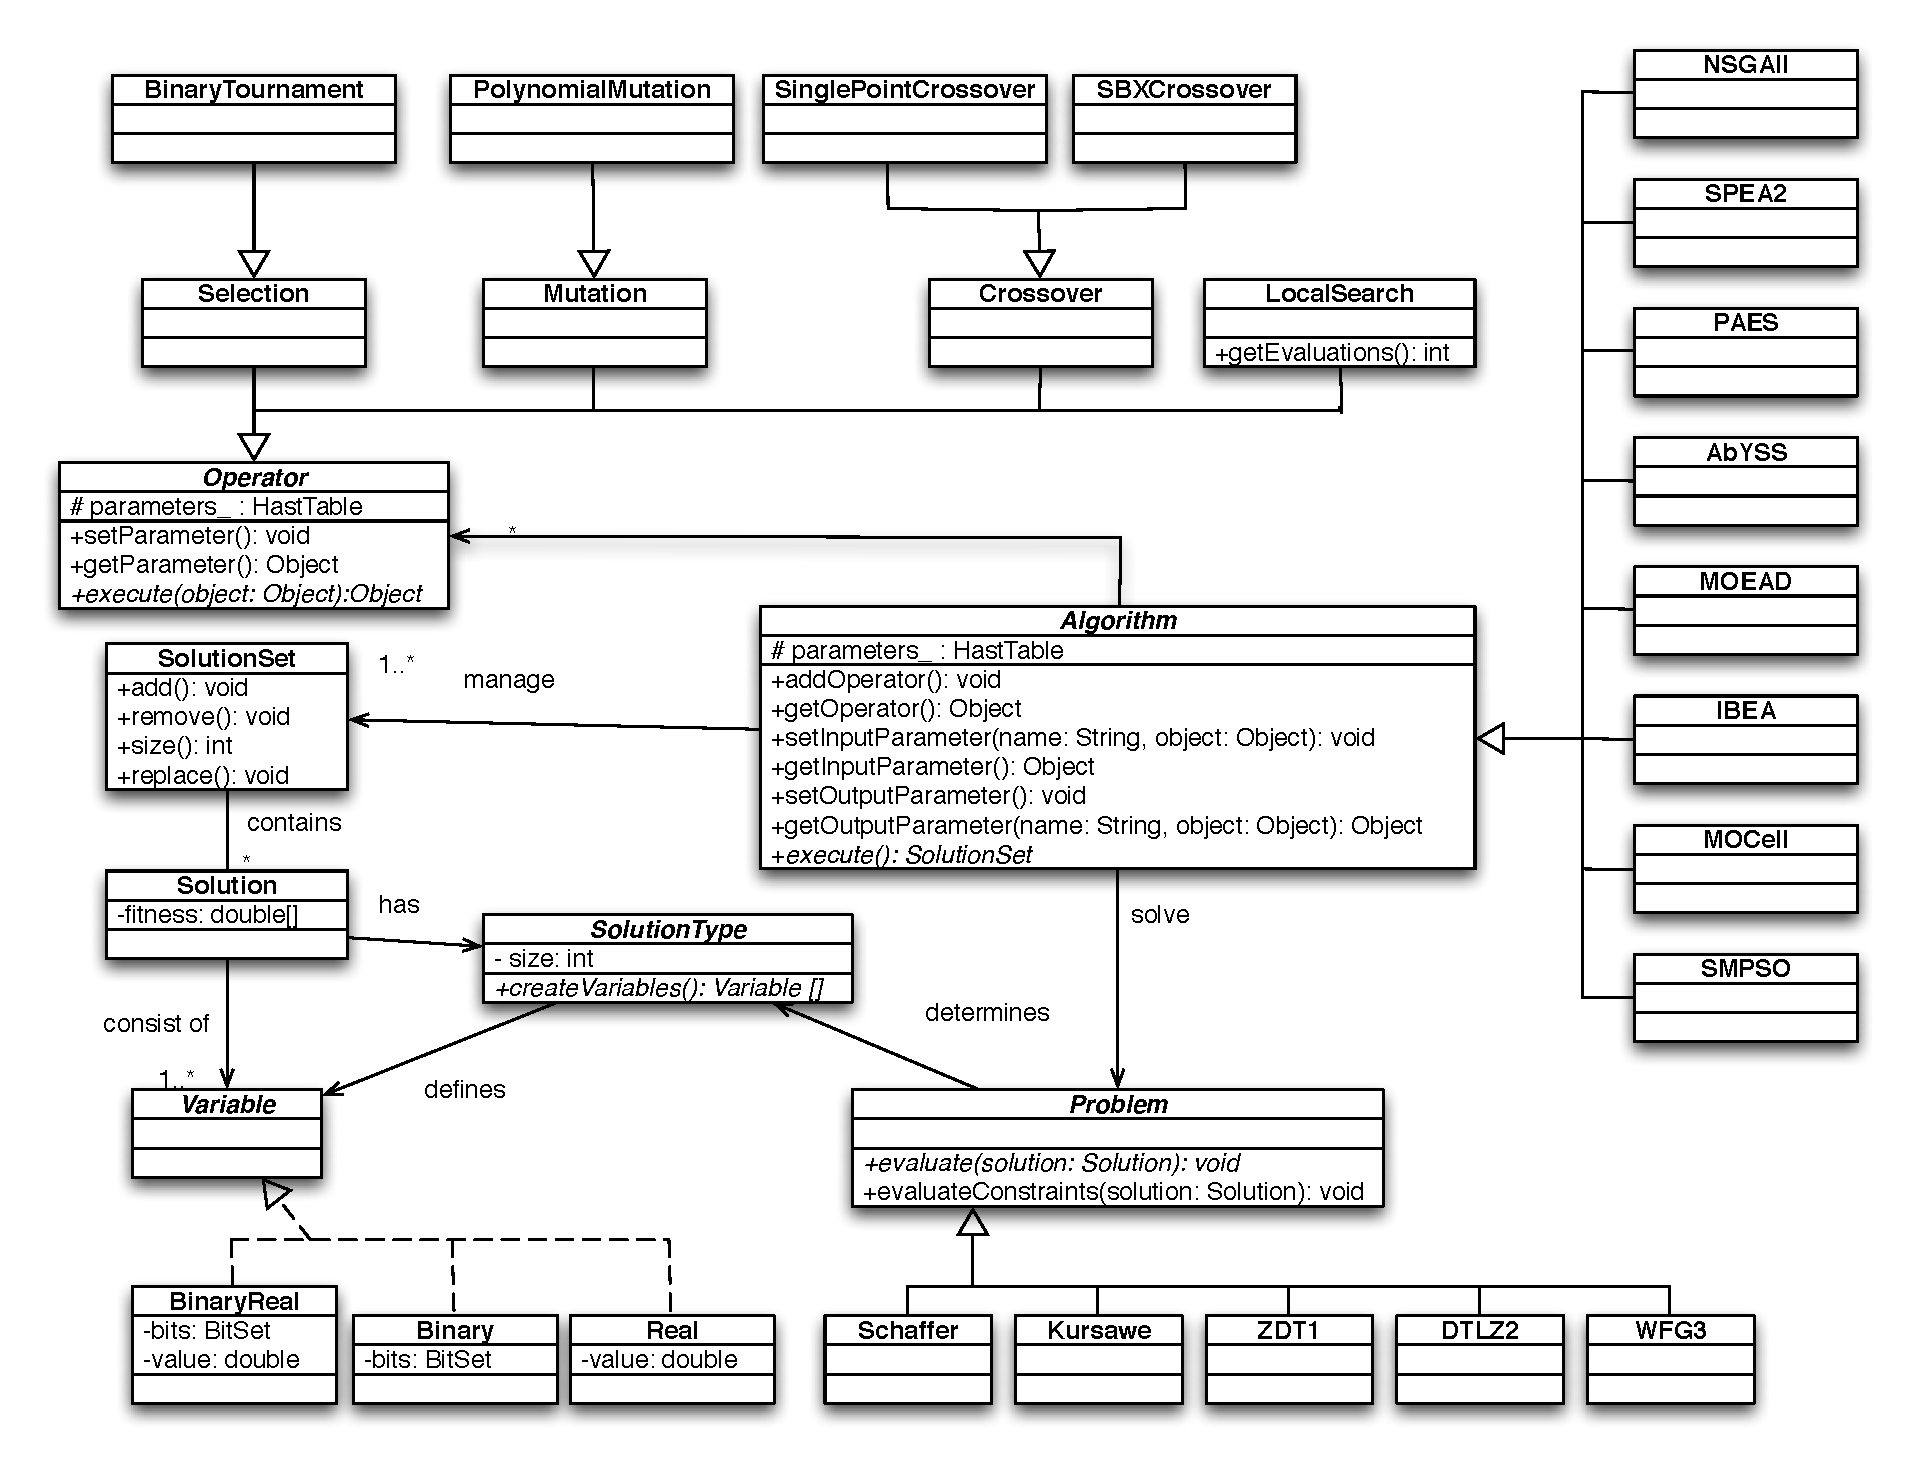
\includegraphics[width=135mm]{img/methodology/jMetalUML.eps}}
	\caption{General architecture of jMetal.}
	\label{fig:architecture} 
\end{figure*}

A generic terminology to name the classes within jMetal was employed in order to make them general enough to be used in any metaheuristic. This way, in the context of evolutionary algorithms, populations and individuals correspond to {\it SolutionSet} and {\it Solution} jMetal classes, respectively; the same can be applied to PSO algorithms concerning the concepts of swarm and particles.

Class {\it Algorithm} represents the superclass for all the optimizers: whatever metaheuristic included in jMetal has to inherit from it. An instance object of {\it Algorithm} may require some application-specific parameters, that can be added and accessed by using the methods {\it addParameter()} and {\it getParameter()}, respectively. Similarly, an algorithm may also make use of some operators. For example, genetics algorithms typically use operators for recombination and selection of individuals. There are also methods for incorporating operators ({\it addOperator()}) and to get them ({\it getOperator()}). The main method in {\it Algorithm} is {\it execute()}, which starts the execution of the algorithm. 

As its name suggests, class {\it SolutionSet} represents a set of {\it Solution} objects. Each {\it Solution} object has associated a type ({\it SolutionType}) and it is composed of an array of {\it Variable} objects. This last is a superclass aimed at describing different kinds of representations for solutions. The proposed scheme by jMetal is very flexible because a {\it Solution} object is not restricted to contain variables of the same representation; instead, it can be composed of an array of mixed variable types. Furthermore, it is also extensible, because new representations can be easily incorporated into the framework, just by inheriting from {\it Variable}.

In jMetal, all the problems have to inherit from class {\it Problem}. This class contains two basic methods: {\it evaluate()} and {\it evaluateConstraints()}. Both methods receive a {\it Solution} representing a candidate solution to the problem; the first one evaluates it, and the second one determines the overall constraint violation of that solution. All the problems have to define the {\it evaluate()} method, while only problems having side constraints need to define {\it evaluateConstraints()}. The constraint handling mechanism implemented by default is the one proposed in~\cite{deb02fast}.

{\it Operator} is a superclass aimed at representing generic operators to be used by the different algorithms (e.g., crossover, mutation, or selection are typical operators in the field of evolutionary algorithms). As {\it Algorithm}, it contains the {\it getParameter()} and {\it setParameter()} methods, which are used for adding and accessing to operator specific parameters. For example, the simulated binary (SBX) crossover~\cite{deb01multiobjective}, employed by many evolutionary algorithms, requires two parameters: a crossover probability (as most crossover operators) plus a value for the distribution index (specific of the parameter). This operator receives as a parameter two parent individuals and, as a result, it returns the offspring resulting of recombining both parents. The use of the generic Java class {\tt Object} allows a high degree of flexibility. Thus, a {\it BinaryTournament} operator, which is a selection operator employed by many genetic algorithms, will receive as a parameter a {\it SolutionSet} object and it will return a {\it Solution} object, while a {\it PolynomialMutation} operator, also a mutation operator typically used in evolutionary algorithms, will receive a {\it Solution} object, will modify this object, and it will return a null value.

A more detailed description of the jMetal architecture can be found in~\cite{DN10jmetal} and in the jMetal user manual~\cite{ND10}.

\section{Integrating jMetal and AutoDock 4.2}
\label{sec:jMetal_Autodock}

jMetal is an open-source framework aimed at multi-objective optimization with metaheuristics, but it also incorporates many algorithms for single-objective optimization. Our idea is to develop a clean integration between jMetal and AutoDock 4.2 in such a way that the algorithms available in jMetal can be used to solve docking problems by using the fitness function provided by AutoDock 4.2 (in the case of mono-objective metaheuristics). This implies that the metaheuristics run in jMetal and, whenever a new solution has to be evaluated, the solution has to be sent to AutoDock, which returns the corresponding binding energy. Once AutoDock has been properly configured, it enters a loop and waits for jMetal evaluation requests; when the algorithm in jMetal finishes, the best solution is sent to AutoDock, which continues its execution as if the incorporated GA or LGA had finished (see Figure~\ref{Fig:integration}). Thus, the final results have the same format and they are familiar to AutoDock users.

\begin{figure*}[!h]%figure_integration
	\centerline{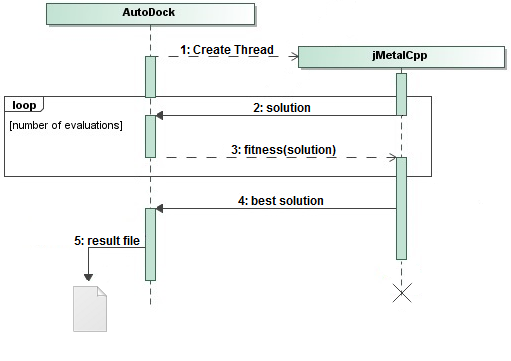
\includegraphics[width=0.70\textwidth]{img/methodology/integration.png}}
	\caption{Sequence diagram which represents the communication between AutoDock and jMetal during a mono-objective algorithm execution. The two threads communicate with each other a number of times, equal to the number of evaluations. Finally, the jMetal thread returns the best solution to the main AutoDock thread.}
	\label{Fig:integration} 
\end{figure*}

In the case of the multi-objective metaheuristics, the integration process is nearly identical but differs in some small details. Instead of getting the binding energy value (fitness) after sending a solution to AutoDock to be evaluated, the code was modified to receive to independents components of that binding energy value: the intermolecular energy and the intramolecular energy. These two values will be treated as two different objectives to be minimized. After finishing all the algorithm iterations, instead of getting one best solution, a front containing a set of non-dominated solutions is obtained. However, one of the solutions contained in the front has to be returned to the AutoDock thread, so the main thread is able to finish as expected (see Figure~\ref{Fig:integration-multi}).

\begin{figure*}[!h]%figure_integration_multi
	\centerline{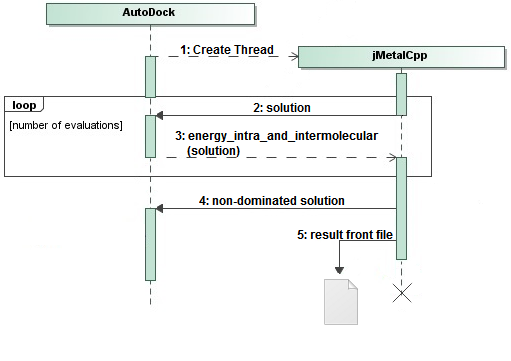
\includegraphics[width=0.70\textwidth]{img/methodology/integration-multi.png}}
	\caption{Sequence diagram which represents the communication between AutoDock and jMetal during a multi-objective algorithm execution. The two threads communicate with each other a number of times, equal to the number of evaluations. Finally, the jMetal thread returns a non-dominated solution to the main AutoDock thread. The entire approximated front is returned by the jMetalCpp thread in an output file.}
	\label{Fig:integration-multi} 
\end{figure*}

In our first attempt, we considered using the JNI framework to directly invoke the AutoDock energy function from jMetal, but AutoDock 4.2 is a rather complex software package, which requires the parameter settings of an experiment to be indicated in a configuration file, and a pre-processing of them is required in order to start running a solver. We therefore decided that a more promising approach was to first configure both packages and then run them in parallel.

As jMetal and AutoDock are coded in different languages, the first integration was done by using sockets for the communication between them; JSON was used as data interchange format. This solution worked, but it was very inefficient, so we took the decision to write a port of a significant subset of jMetal to C++ from scratch. The adopted solution consists of running AutoDock and jMetal in two different threads inside the same process, so they communicate by sharing memory and synchronize with mutexes (see Figure~\ref{Fig:integration} and Figure~\ref{Fig:integration-multi}). This approach is efficient and flexible, allowing any of the algorithms included in jMetal to be easily used for solving docking problems.